\chapter{Lecture 18 - Scientific visualization}

\begin{definition}[Scientific visualization]
    Scientific visualization is defined as the study of computing techniques used to generate interactive visual representations of acquired or simulated spatio-temporal data.
\end{definition}

The modern process takes raw data, often generated in massive sizes by sensor computer simulations, and convert it into a form that is understandable to humans. Because data sizes are increasing exponentially, a graphical approach is often the only way for researchers to identify patterns and interpret results effectively. A key component of this field is the development of efficient algorithms for the interactive manipulation and exploration of data. This allows scientists to move through their data, change parameters, and explore scientific features in real-time.

\section{Basics}

\begin{definition}[Dataset]
    A dataset is defined as a pair consisting of a domain and attributes. This relationship is expressed mathematically as a function \(f: D -> A\), where:\par
    Domain \(D\) is the input geometrical object or physical space being studied\par
    Attribute \(A\) is the specific data values (co-domain) defined at each point of that domain
\end{definition}

The specific visualization technique chosen depends entirely on the type of domain and the mathematical nature of the function.

\subsubsection{The nature of domain}
Data is typically represented by a finite set of samples. To treat this as a continuous field, the system uses interpolation schemes to estimate values between those samples. A domain is characterized by its dimension (2D surface or 3D volumes), embedding (positional information in space), and connectivity (information about how the data points are linked together).

\subsubsection{Domain discretization}
Domains are categorized based on their internal structure and connectivity: 
\begin{itemize}[noitemsep]
    \item Structured domains: these use fixed connectivity, often in the form of a grid (uniform grid, rectilinear grid, curvilinear grid)
    \item Unstructured domains: these have arbitrary connectivity and irregular geometry. It can be unstructured points, also called point clouds, with no explicit connectivity information; or unstructured grids that use irregular combinations of cell with mesh being the most popular choice.
\end{itemize}

\subsubsection{The nature of attributes}
Attributes represent the actual scientific measurement and are classified by their co-domain dimension: scalar (single value, like temperature), vectors (values with both magnitude and direction, like velocity), and tensors (complex multi-dimensional attributes). \par
Attributes can be deterministic (exact measurements) or uncertain (often resulting from ensemble observations in simulations), with the visualization of uncertain data being a specialized branch of research.

\section{Scalar field visualization}
Scalar field visualization is used when the attributes at every point in a domain are represented by a single numerical value, such as density, pressure, or temperature.\par
The most intuitive way to visualize scalar values is by mapping them to perceptual channel, specifically color. The color map is a palette of colors arranged continuously and mapped to the real line. Every scalar value in the dataset is then assigned a corresponding color from this palette to produce a visual field.

\subsubsection{Transfer function and classification}
When dealing with 3D volumes, simple color mapping is not enough because the "inside" of the object would be hidden. To overcome this, researchers use \textbf{transfer functions}, which map scalar values not just to color, but also to opacity (transparency). This process of assigning specific colors and transparency levels to different data densities is known as \textbf{classification}. For example, in a medical scan, a transfer function might make "air" transparent, "muscle" semi-transparent, and "bone" opaque and white.\par
Designing effective transfer functions is difficult and often requires domain-specific knowledge, though semi-automatic tools like "design galleries" exist to help.

\subsubsection{Volume rendering}
The overall process of mapping a 3D scalar field to color and transparency to create a final image is called \textbf{volume rendering}. A common technique is \textit{volume ray casting}, where the system shoots rays through the data, each point or cell along the ray contributes to the final pixel color, and these contributions are blended together through mathematical integration.

\subsubsection{Geometric and topological features}
Beyond just coloring the data, scalar fields are often analyzed by identifying specific geometric features:
\begin{itemize}[noitemsep]
    \item Isolines and isosurfaces: these are sets of points where the scalar field has the same constant value (llike contour lines on a map). Isolines are used for 2D surfaces, while isosurfaces are used for 3D volumes
    \item Critical points: in a smooth mathematical setting, critical points are locations where the gradient of a scalar function vanishes. These points characterize the shape of the field, including maxima, minima, and saddles.
\end{itemize}

\subsubsection{Morse function}
A smooth function is called Morse function if all of its critical points are non-degenerate (meaning they are isolated and well-behaved). Morse theory is powerful because it establishes a direct relationship between these critical points and the overall topology of the manifold.

\subsection{Piece-wise Linear (PL) setting}
In practical scientific visualization, data is rarely a smooth function; instead, it is a PL scalar field where values are provided at vertices and interpolated elsewhere.\par
Because the gradient is constant within each triangle (simplex) in a PL mesh, the standard definition of a critical point doesn't work. To find critical points on a mesh, researchers look at the connectivity of a vertex's lower link (neighboring vertices with lower values) and upper link (neighbors with higher values). A vertex is regular if both links are simply connected; otherwise, it is a critical vertex.

\begin{figure}[htbp]
    \centering
    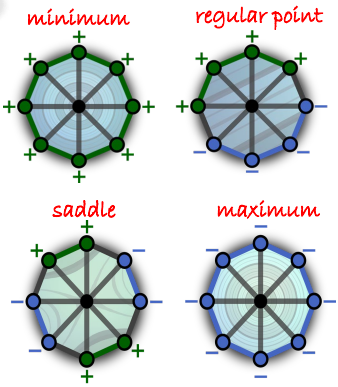
\includegraphics[width=0.4\linewidth]{imgs/lecture18/18.1 critical points.png}
    \caption{Critical points on PL scalar field}
    \label{fig:18.1}
\end{figure}

\subsubsection{Reeb graph}
A Reeb graph is a 1D "skeleton" used to track the evolution of level sets (contour) as the scalar value changes. It contracts each connected component of a level set into a single point. The topology of level sets changes at critical points, while extreme (maxima/minima) map to valence-1 vertices in the graph, saddle points appear as points where the graph branches or merges.

\subsubsection{Noise and persistence}
In real-world data, noise can create many, tiny "fake" critical points. To filter these out, a simple mechanism to classify critical points as either noise or signal, the \textbf{Persistent Homology}:
\begin{itemize}[noitemsep]
    \item \textbf{Filtration}: the system looks at a sequence of "sub-level sets" as the function value increases, noting when topological features (like components or holes) appear and disappear.
    \item \textbf{Persistence}: it is the absolute value of f-value difference of critical points pairs. The importance of a feature is measured by its lifespan (the difference in values between its birth and death). This can provide a concise representation of critical point pairs, but they do not provide info on the adjacency relations of pairs on the domains.
    \item \textbf{Topological simplification}: by using a persistence diagram, researchers can identify features with low persistence (noise) and remove them to create a simplified, cleaner representation of the data.
\end{itemize}

\section{Vector and Tensor visualization}
In a vector field, each data point contains a vector, which is characterized by both a magnitude and a direction. Common examples include tracking the rate of changes in a system, deformations caused by physical forces, or velocity in fluid dynamics. 

\subsubsection{Vector field visualization - Drawing arrows}
The most straightforward way to visualize these fields is by drawing arrows at sample points. Magnitude is typically mapped to the arrow's length, width, or color. This method requires no interpolation and provided a quick overall impression of the field. But it can suffer from occlusion (arrows blocking each other) and perspective distortion in 3D, which may require user interaction to correctly perceive depth cues. 

\subsubsection{Flow-based techniques}
To provide a more integrated view of how the field behaves, researchers use curves that follow the flow:
\begin{itemize}[noitemsep]
    \item Streamlines: these are families of curves that are tangent to the vector field at every point, showing the path a particle would take through the flow
    \item Advanced geometries: to provide more visual information, streamlines can be expanded into stream-ribbons, stream-tubes, or stream-surfaces.
    \item Topological analysis: similar to scalar fields, vector fields can be analyzed using topological data analysis, such as the Morse-Smale Complex, to identify the core structural skeleton of the flow. 
\end{itemize}

\subsubsection{Tensor field visualization}
Tensors represent even more complex attributes, often involving derivatives of vector fields. These are critical for solving problems in mechanics (such as stress or strain) and in medical imaging. Because tensors are multi-dimensional, visualizing them requires sophisticated glyphs or textures that can represent multiple values at a single point simultaneously.

\section{Scientific illustration}
\begin{definition}[Scientific illustration]
    Scientific illustration is a discipline that renders images of scientific subjects to inform and communicate complex ideas. It combines aesthetic skill with scientifically informed observations to portray what is often "unobservable", ranging from the internal anatomy of arthropods to molecular structures and geological cross-sections.
\end{definition}

While traditional computer graphics often strive for photorealism, \textbf{Non-Photorealistic Rendering} (NPR) is inspired by traditional artistic media like painting, drawing, and cartoons. The goal is to use abstraction to highlight specific features of a model that might be lost in a realistic render. The key techniques include:
\begin{itemize}[noitemsep]
    \item Sparse line drawing: these use a minimal set of linear contours to illustrate the primary features and edges of an object
    \item Stippling: this involves creating patterns using small dots to simulate different degrees of shading, solidity, and volume.
\end{itemize}

\begin{figure}[htbp]
    \centering
    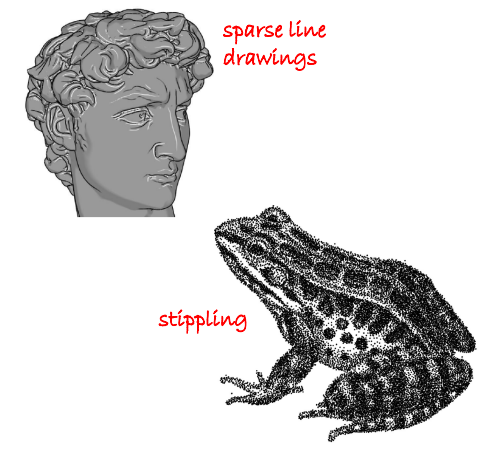
\includegraphics[width=0.5\linewidth]{imgs/lecture18/18.2 NPR.png}
    \caption{NPR techniques}
    \label{fig:18.2}
\end{figure}

\subsubsection{Expressive visualization}
To better show the internal structure or the relationship between different parts of a complex object, the expressive visualization techniques can be used, such as \textit{cut-way illustrations} (remove parts of an outer shell to reveal what is hidden inside), or \textit{explosion diagram} (separate the components of an object while maintaining their relative orientation to show how they fit together).

\begin{figure}[htbp]
    \centering
    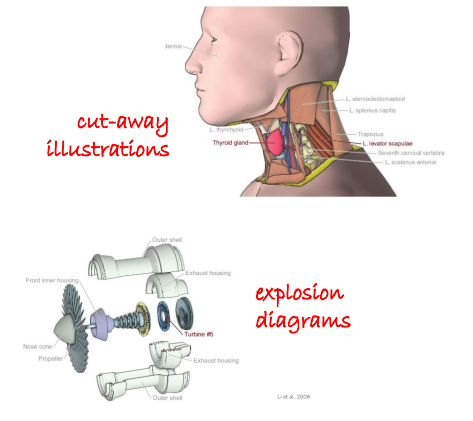
\includegraphics[width=0.5\linewidth]{imgs/lecture18/18.3 expressive visualization.png}
    \caption{Expressive visualization techniques}
    \label{fig:18.3}
\end{figure}

\section{Physical reproduction}
The tangible nature of physical models triggers different cognitive and perceptual processes than purely visual stimuli. These reproductions allow for the direct manipulation of spatial relationships.\par
In learning environments, tangible 3D molecular models can help students conceptualize complex phenomena in a more engaging and stimulating format than computer-generated graphics alone. 

\subsection{SW tools}
There are two primary SW environments used by professionals, Paraview (an open-source application designed for visualizing both 2D and 3D datasets) and TTK - Topology ToolKit (A specialized toolkit for performing the topological analysis including generation of Reeb graphs and persistence diagrams).

\section{Case study - Coral phenotyping}
Traditionally, marine biologists took measurements underwater using metric cords and waterproof notebooks, a process that was often impractical, imprecise, and potentially destructive to the coral. The researchers proposed replacing this with 3D digital replicas. The workflow:
\begin{itemize}[noitemsep]
    \item Reconstruction: underwater photographs are used to reconstruct a high-detail 3D mesh
    \item Analysis: using geometry processing, the system computes a skeletal structure that follows the coral's morphology
    \item Segmentation: this tool identifies and segments single coral branches, ordering them into a parent-child hierarchy from the root to the tips
    \item Measurements: ecologists can then cut the branches digitally to compute critical measures such as length, angles, surface areas, and volumes.
\end{itemize}

This method provides a permanent recording of the coral that can be measured repeatedly over time without further disturbing the environment.